\chapter{Impact of vegetation on the airflow}
\def\figdir{chapters/ch04_experimentalstudymodels/figures}

\textit{This chapter is based on paper \cite{Manickathan2018b}}.

\section{Introduction}

\lettrine[lines=3,nindent=0em,loversize=0.1]{T}{h}is chapter focuses on assessing the impact of vegetation on the airflow from experimental observation. The paper, \cite{Manickathan2018b}: ``\textit{Comparative study of flow field and drag coefficient of model and small natural trees in a wind tunnel}'' assists in revealing the impact of vegetation on the airflow. In the study, at first the airflow of model trees are compared with the ones of natural trees of a similar size to determine whether both types of tree provide similar aerodynamic characteristics. Thereafter, the flow field and drag coefficient of model trees are compared to the ones of natural trees of similar size to determine whether model trees can be used to represent natural trees. And, the drag coefficient of small model trees and natural trees are compared with the ones measured on larger natural trees in literature. The study investigates the sheltering provided by small model trees and how it differs from that of small natural trees. Furthermore, the study investigates the influence of season foliage density change of a natural tree and how it impacts the drag coefficient and subsequently the flow field in the wake.

\section{Background}

Wind tunnels provide a controlled setup, enabling detailed studies on the impact of tree properties, such as porosity and flexibility, on drag. \cref{tab:windtunneltreeslit} briefly summarizes previous studies of drag forces on model and natural trees in wind tunnels. The natural trees are categorized into two types: hardwood and coniferous species. In these studies, the drag measurements are performed under airflow varying between $4$ and $20$ m\,s$^{-1}$. The main limitation of wind tunnel measurements is the height of the wind tunnel, as it restricts the maximum size of the measured trees. Nevertheless, these controlled experiments provide an improved understanding of the influence of tree morphology on the drag coefficient. They can improve the computational fluid dynamics (CFD) modelling of vegetation and respective model calibration, and thereby enable a more accurate assessment of the impact of vegetation on the environment \citep{Bitog2011,Bitog2012}. Additionally, wind tunnels enable non-intrusive flow measurements of the tree wake using particle image velocimetry (PIV). Such PIV measurements of the wake allow quantifying the impact on turbulence and the degree of sheltering provided by trees \citep{Lee2012,Lee2014565}.

{
	\ctable[
	caption = {Summary of previous studies measuring the drag coefficient of model and natural trees in wind tunnel.},
	label   = {tab:windtunneltreeslit},
	pos = p,
	mincapwidth = \textwidth,
	sideways,
	]{llrrl}{Scientific names: $^a$\textit{Thuja occidentalis Smaragd}, $^{b}$\textit{Hibiscus syriacus}, $^{c}$\textit{Thuja plicatas},\\
		$^{d}$\textit{Tsuga heterophylla}, $^{e}$\textit{Pinus contorta}, $^{f}$\textit{Alnus rubra}, $^{g}$\textit{Populus tremuloides}
	}{
		
		\FL
		Tree type 				&	Species 		 & 		$H$ (m) 		& $U$ (m\,s$^{-1}$) & References
		\ML
		model					& 	wood-wool		 & $0.115$ & $5.5 - 13.5$ & \multirow{2}{*}{\cite{Gromke2008a}} \\
		model					& 	sisal-fibre		 & $0.115$ & $5.5 - 13.5$ & 	\\[7pt]
		coniferous				& 	emerald cedar$^a$	 & $0.98$~~	& $5 - 15$~~~ & \multirow{2}{*}{\cite{Cao2012}} \\
		hardwood				& 	rose of sharon$^b$   & $1.24$~~	& $5 - 15$~~~ &  \\[7pt]
		coniferous				& 	western redcedar$^c$ & $1.95$~~	& $4 - 20$~~~ & \multirow{3}{*}{\cite{Vollsinger2005a}} \\
		coniferous				& 	western hemlock$^d$  & $1.95$~~	& $4 - 20$~~~ & \\
		coniferous				& 	lodgepole pine$^e$   & $1.95$~~	& $4 - 20$~~~ & \\[7pt]
		hardwood				& 	red adler$^f$   	 & $1.95$~~	& $4 - 20$~~~ & \multirow{2}{*}{\cite{Vollsinger2005}} \\
		hardwood				& 	trembling aspen$^g$	 & $1.95$~~	& $4 - 20$~~~ & 
		\LL}
}

Atmospheric boundary layer wind tunnel studies focus on trees in an urban setting \citep{Gromke2011,Gromke2008a}, measurements of flow past windbreaks \citep{Guan2003} or in forest canopies \citep{Bai2013,Conan2015,Kinnersley1994}, but are limited to the use of small model trees to match the size of building models typically used in these wind tunnel studies. This requirement prohibits the use of a larger mature natural tree. However, it is not known sufficiently to which extent small model trees can substitute such natural trees and whether both types display similar aerodynamic characteristics. There are several difficulties associated to scaling down of large natural trees to smaller model trees. Natural trees vibrate, deform and reconfigure, which all directly influence the drag and the resulting flow field around the tree \citep{Schouveiler2006,Tadrist2014,Vogel1989}. The mechanical properties of the tree are known not to scale linearly with size, so this fact should be considered when employing smaller trees to represent their larger counterparts \citep{DeLangre2008}. Moreover, predicting the dynamic response of a natural tree itself is a complex task due to the anisotropy in the material properties of the plant \citep{James2017}. The tree trunk wood of natural trees are known to have a radial anisotropy, resulting in a more complex mechanical response compared to isotropic materials \citep{Albrecht2016}. Furthermore, the location of the plant during its growth, for example forest-grown trees versus isolated trees, is known to alter the final form of the canopy architecture (James et al., 2014). Therefore, the plant growth history also plays a vital role in the plant morphology, and will result in a different mechanical response. Moreover, the age of the plant, varying from juvenile sapling to a mature plant, will further influence the mechanical properties of the plant. In this context, various authors have shown that the elastic modulus varies not only with species but also with the maturity of the plant \citep{Dahle2010,Macdonald2002,Telewski1995,Watt2008,Woodrum2003}. It is challenging to capture such allometric and morphological variability of different plants with small model trees. Without adequate care when designing the model trees, the response of model trees will not exactly represent natural trees that are found in an urban environment.

\section{Model and Natural trees}

A range of model and natural trees with different heights and porosities is used in the present study to answer questions regarding whether model trees behave similarly to natural trees. \cref{tab:modeltrees} lists the specification of the model and natural trees used for drag and PIV measurements. It tabulates the tree type, tree height $H$, frontal area $A$, optical porosity $\beta$ and aerodynamic porosity $\alpha$. The aerodynamic porosity $\alpha$ is determined directly from the optical porosity $\beta$ using an empirical relationship:
\begin{equation}
\alpha = \beta^{0.4}
\label{eq:aerodynamicporosity}
\end{equation}
obtained from a wind tunnel drag study of realistic tree-like windbreak models \citep{Guan2003}. The study shows that this formulation provides a good estimate for 3D tree models and has been applied by others to estimate the aerodynamic porosity for individual trees \citep{Bitog2011,Lee2014565,Rosenfeld2010}.

	\begin{figure}[t]
	\centering
	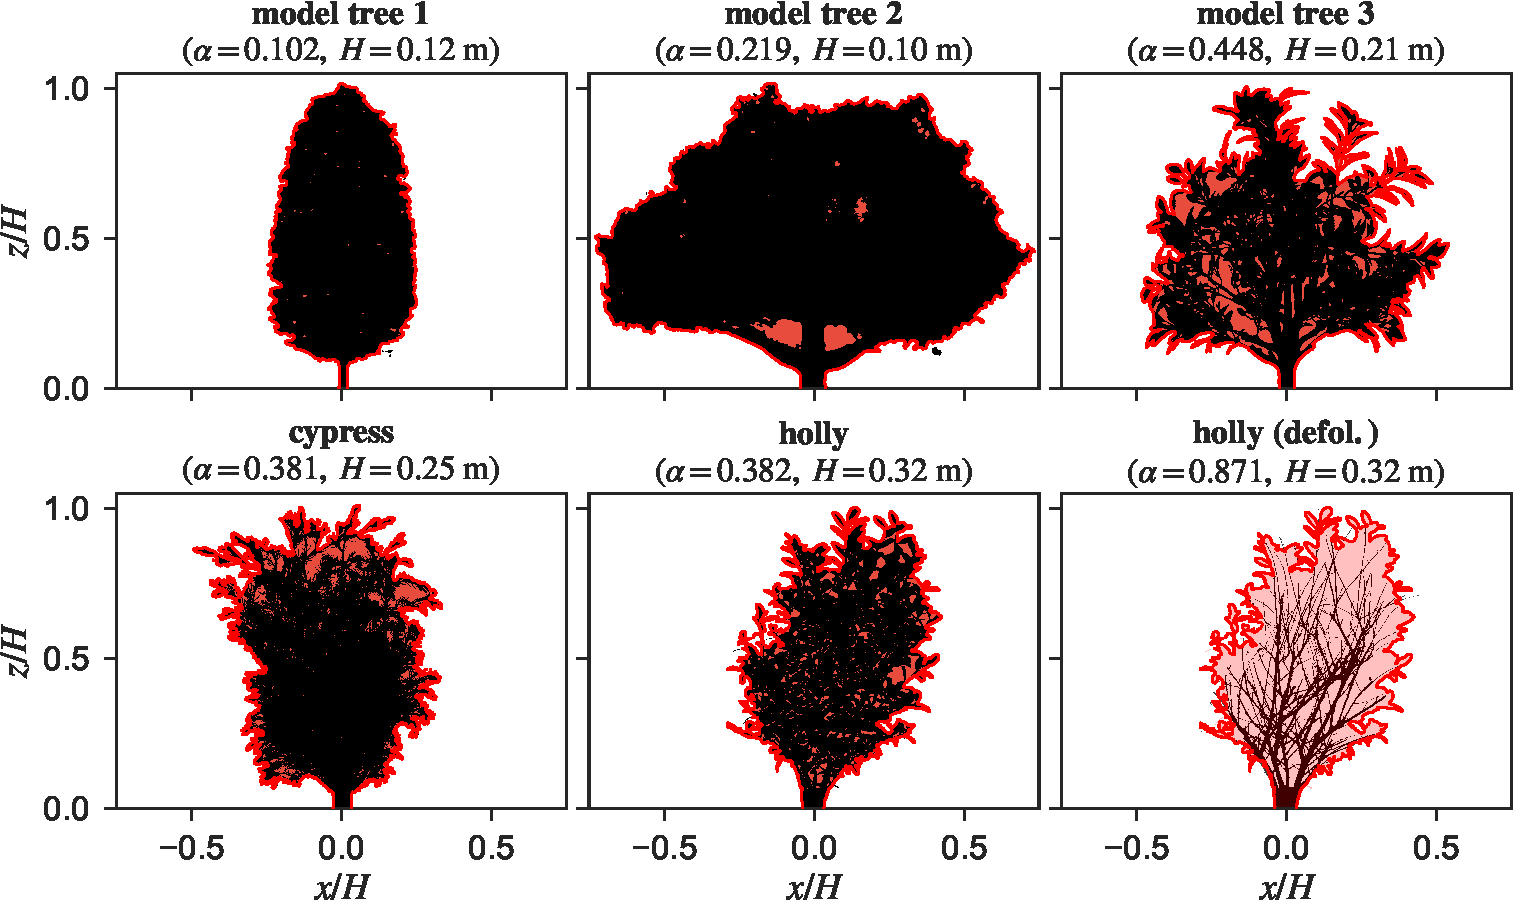
\includegraphics[width=\textwidth]{\figdir/threshold_indexed-crop.pdf}
	\caption{Frontal thresholded images of model and natural trees at rest: \subfig{a} model tree 1, \subfig{b} model tree 2, \subfig{c} model tree 3, \subfig{d} cypress, \subfig{e} holly and \subfig{f} holly (defoliated). The red region indicates the frontal area of the tree. The frontal area of holly is used as a reference for both foliated and defoliated holly.}
	\label{fig:thresholdindexed}
	\end{figure}

\cref{fig:thresholdindexed} shows the thresholded frontal view of the model and natural trees used during the experiment. The thresholded images are used for the calculation of optical porosity and the resulting aerodynamic porosity. The optical porosity is defined as the ratio of the number of white pixels to the total number of pixels within the silhouette of the tree, which is delineated in red on \cref{fig:thresholdindexed}. To note is that this silhouette area is considered as the frontal area of the tree $A$ used in \cref{eq:aerodynamicporosity} and also required for calculating the drag coefficient $C_d$ (further explained in \cref{subsec:loadcell}). The drag measurements are performed for all the trees listed in the table and PIV measurements are performed for a selected number of trees (two model and two natural trees as indicated in \cref{tab:modeltrees}. These trees are chosen based on their distinct differences in morphology and porosity. Model trees 1 and 2 are small model trees made of polymeric materials with different porosity and shape. These are H$0$ scale (a standardized scale of 1:87 for rail transport modeling) broad-leaf model trees. Model tree 3 is a larger model, with individual polymeric thin leaves mimicking those of a natural tree. The model trees are commercially available and have been designed to capture the geometrical characteristics of the natural trees. Such scaled models are typically used in wind-tunnel studies of urban microclimate research, to represent the impact of trees on the airflow field around scaled model buildings \citep{Gromke2018a,Gromke2008,Gromke2007,Guan2003,R.N.Meroney1968}. Note however that designing trees to match the mechanical properties of the actual trees of interest would be most realistic. The design of model trees that have the mechanical properties of the natural trees such as moment of elasticity (MOE) or the bending stiffness requires careful design. In the past, various types of materials such as plastic-simulated boughs \citep{R.N.Meroney1968}, Nylon-66 stems with low-density Polyethylene (LDPE) branches \citep{Stacey1994} have been used to provide flexibility to the tree models. Tree models with crowns made of wood-wool, sisal fiber or porous foam on a stiff trunk \citep{Gromke2008a} have also been designed to provide appropriate porosity and drag coefficient. Even though rigid model trees can be deemed appropriate to capture the static response, the dynamic response of the natural trees is not captured due to their rigidity. Therefore, one of the objectives of the study is to see to which extent the flexible model trees, such as H$0$ scale trees, can provide more accurate airflow fields for wind tunnel studies, due to their flexibility. 

	\ctable[
caption = {Specifications of the model and natural trees used for drag and PIV measurements. The trees used for PIV measurements are indicated with an asterisk (*).},
label   = {tab:modeltrees},
pos = t,
mincapwidth = \textwidth,
]{llrrrr}{ $^{(1)}$ \cite{Guan2003} \\
	Scientific names: $^a$\textit{Chamaecyparis pisifera}, $^{b}$\textit{Ilex crenata}
	}{	\FL
		Name	 				&	Tree type 		 & $H$ (m) 	& $A$ (cm$^2$) 	& $\beta$ 	& $\alpha$ $^{(1)}$
		\ML
		model tree 1 (*)		& 	model			 & $0.12$ 	& $48$ 			& $0.003$ 	&	$0.102$	 \\
		model tree 2 			& 	model			 & $0.1$~~ 	& $82$ 			& $0.022$ 	&	$0.219$	 \\		
		model tree 3 (*) 		& 	model			 & $0.21$ 	& $240$ 		& $0.134$ 	&	$0.448$	 \\		
		cypress$^{a}$ (*)		& 	coniferous		 & $0.25$ 	& $297$ 		& $0.09$~~ 	&	$0.381$	 \\						
		holly$^{b}$ (*)			& 	hardwood		 & $0.32$ 	& $411$ 		& $0.09$~~ 	&	$0.382$	 \\								
		holly$^{b}$ (defol.) (*)	& 	hardwood	 & $0.32$ 	& $411$ 		& $0.708$		& $0.871$							
		\LL}

The natural trees used in the present study are divided into two categories: hardwood and coniferous species. Generically, hardwood species have broad-like leaves whereas coniferous trees have needle-like leaves. In the present study, smaller young (juvenile) trees are used with a maximum height of $32$ cm, although a typical mature holly is known to grow up to \numrange{3}{5} m and a mature cypress to \numrange{35}{50} tall. The impact of seasonal foliar density variation is studied by defoliating the holly and subsequently performing drag and flow measurements.

	\begin{figure}[t]
	\centering
	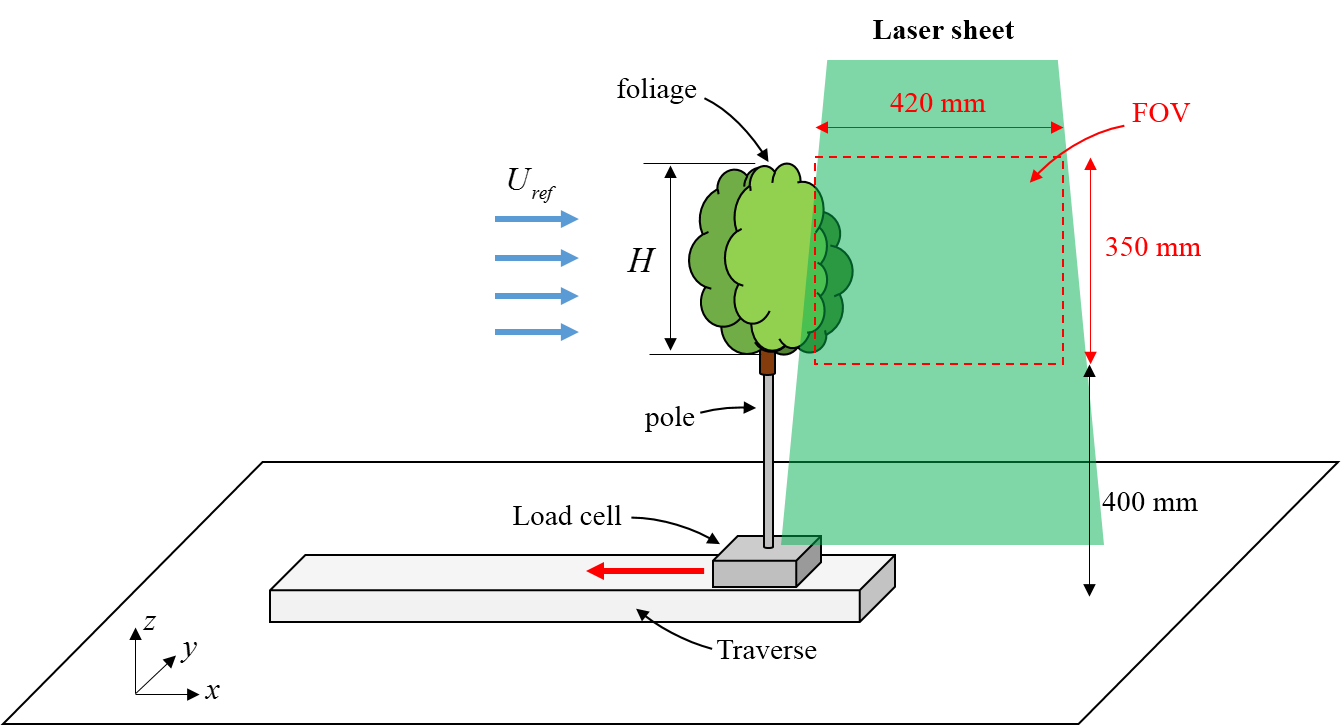
\includegraphics[width=\textwidth]{\figdir/setup_image.png}
	\caption{Wind tunnel setup for combined drag force and PIV measurements. The model trees or natural trees are positioned on a rigid stainless steel pole connected to the load cell. The trees are traversed 3 times in the upstream direction by $300$ mm, indicated by the red arrow.}
	\label{fig:setupimage}
	\end{figure}

The wind tunnel experiments are performed in the ETHZ / Empa Atmospheric Boundary Layer (ABL) wind tunnel. It is a closed circuit G\"ottingen type wind tunnel with a test section cross-section of $1.9$ m (width) by $1.3$ m (height). The wind tunnel can provide wind speeds ranging from \numrange{0.5}{25} m\,s$^{-1}$. \cref{fig:setupimage} shows the setup used for combined measurement of drag force and the flow field behind the trees. The origin of the $x$, $y$, $z$  coordinate system is located at the bottom-center of the tree foliage. The corresponding instantaneous velocity components of the velocity vector $\mvec{u}$ are $u$, $v$, and $w$, oriented along the streamwise, spanwise and vertical directions, respectively. The mean and fluctuating velocities of the velocity vector $\mvec{u}$ are defined $\tavg{\mvec{u}}$ and $\mvec{u}'$, with the overbar denoting an ensemble average. The tree is mounted on the pole-load cell configuration, away from the wind tunnel floor. The trees are mounted in this fashion to reduce the influence of the wind tunnel boundary layer, the load cell and the traverse system at the measurement region. \cref{fig:profiles} shows the normalized mean velocity and the turbulence intensity for two wind speeds of $U_{\textit{ref}}=1$ and $10$ m\,s$^{-1}$. \cref{fig:profiles}a displays a nearly-uniform approach flow wind profile, with a maximum deflection from the mean value less than \num{5e-3} m\,s$^{-1}$. Furthermore, the measurement was performed for a low upstream turbulence with an average turbulence intensity of $I=0.4$\% (\cref{fig:profiles}b). A nearly-uniform wind profile with a low turbulence level is used instead of an atmospheric boundary layer (ABL) to ensure that all trees, which have varying heights, are subjected to the similar velocity profile.

	\begin{figure}[t]
		\centering
		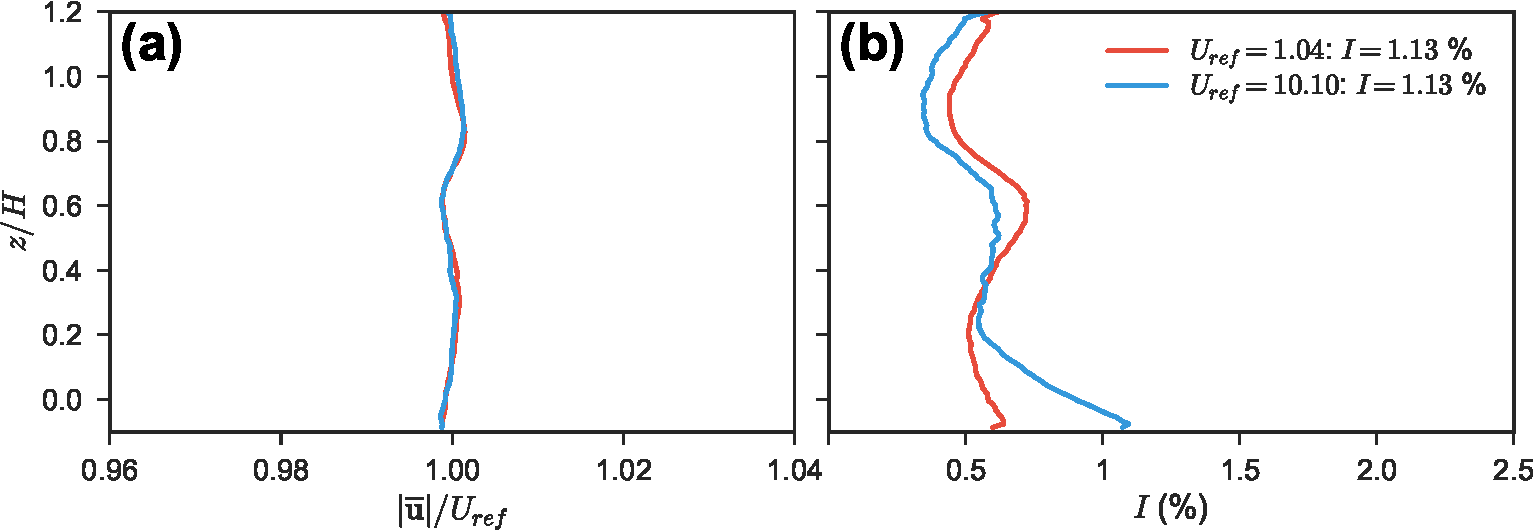
\includegraphics[width=\textwidth]{\figdir/profiles-crop.pdf}
		\caption{Profile at the location $x=0$ m without trees: \subfig{a} normalized mean velocity magnitude $|\tavg{\mvec{u}}|/U_{\textit{ref}}$ and \subfig{b} turbulence intensity $I$ (\%).}
		\label{fig:profiles}
	\end{figure}

\section{Measurement setup}

\subsection{Load cell}
\label{subsec:loadcell}

The force acting on the trees is measured using a Transmetra K3D120-50N 3-axis load cell with a precision of $\pm \num{0.5e-2}$ N. The mean load acting on the tree is determined by averaging over approximately one minute. As the measurement time series is acquired at $2.5$ Hz, the samples are uncorrelated and a sufficiently large sample series is measured. The influence of wind speed on drag coefficient is studied by measuring at six different wind speeds $U_{\textit{ref}} = 3$, $5$, $7$, $10$, $15$ and $20$ m\,s$^{-1}$. A minimum wind speed of $3$ m\,s$^{-1}$ is required due to the resolution of the load cell. The maximum measurement error of $25$\% is found for the smallest model trees at the lowest wind speed due the precision of $\pm \num{0.5e-2}$ N and the averaged measured drag force of \num{2e-2} N. However, with increasing tree size and/or increasing wind speed, the error in the measured drag force quickly reduces to less than $5$\%. The drag coefficient $C_d$ of the trees for a given reference wind speed $U_{\textit{ref}}$ (m\,s$^{-1}$) is given as:
\begin{equation}
C_d = \frac{2F}{\rho U_{\textit{ref}}^2 A}
\label{eq:dragcoefficient}
\end{equation}
where $F$ (N) is the measured drag force in the direction of the wind speed, $\rho$ (kg\,m$^{-3}$) air density and $A$ (m$^{2}$) projected frontal area \citep{Grant1998,Guan2003,Mayhead1973}. As mentioned above, the projected frontal area is calculated directly from the thresholded images of the trees at rest \cref{fig:thresholdindexed}. The frontal area of foliated holly is used as the reference frontal area for the defoliated configuration. This is to ensure that the defoliation of the plant results in an increase in the aerodynamic porosity. If the frontal area is also altered, it can inversely compensate the increase in aerodynamic porosity due to defoliation. The characteristics of the trees are tabulated in \cref{tab:modeltrees}.

\subsection{Particle Image Velocimetry}

The flow field downstream of the trees is measured using particle image velocimetry (PIV). \cref{fig:setupimage} depicts the PIV set-up for measuring the $x-z$ plane at $y=0$ m (defined as the middle of the tree trunk). The PIV set-up consists of a $2560 \times 2160$ pixel ($5.6$ MP) s-CMOS HiSense Zyla camera which images the 1 $\mu$m Di-Ethyl-Hexyl-Sebacat (DEHS) tracer particles, dispersed in the airflow. The particles are illuminated by a $200$ mJ/pulse (at $15$ Hz) Nd-YAG Litron laser. The field of view (FOV), which the camera set-up provides, is $420 \times 350$ mm$^2$. To image the entire recirculation zone of the trees, the tree set-up is traversed 3 times in the upstream direction by $300$ mm, as indicated by the red arrow in \cref{fig:setupimage}. The result is three FOVs with an overlap of $120$ mm that are then stitched together to provide a larger resolved FOV of $1020 \times 350$ mm$^2$. The velocity vectors are calculated using an iterative cross-correlation algorithm of the Dantec DynamicStudio software and the interrogation windows are automatically deformed based on local particle density and velocity gradients. The final interrogation area is $32 \time 32$ px$^2$ with $50$\% overlap. The velocity vector outliers are removed using the normalized median test (Westerweel and Scarano, 2005). For each measurement case, around $200$ samples of statistically independent vector maps are obtained to ensure proper turbulence statistics. The amount of flow field images that are taken ensures a confidence level of $95$\% and leads to the estimation that the maximum free-stream normalized turbulence intensity $I=40$\% in the wake of the trees. During the experiment, the turbulence intensity for all trees is checked not to exceed this upper bound. The sampling rate is based on the largest time-scale determined from the tree height $H$ and the reference wind speed $U_{\textit{ref}}$. For smaller trees ($H=0.1$ m) and larger trees ($H=0.3$ m), at $U_{\textit{ref}}=1$ m\,s$^{-1}$, a sampling rate below $5$ Hz and $1$ Hz is required, respectively.

The PIV measurements were performed for two wind speeds, $U_{\textit{ref}}=1$ and $10$ m\,s$^{-1}$, providing a comparison for low and high wind speeds. The measurements are performed for two model trees and two natural trees (indicated in \cref{tab:modeltrees}) as shown in \cref{fig:thresholdindexed}.

\section{Drag coefficient of model and natural trees}

The drag coefficient is determined using the approach described in \cref{subsec:loadcell}. \cref{fig:cdvswindspeed} shows the drag coefficient of model (dashed colored lines) and natural trees (solid colored lines) as a function of wind speed. Results from previous studies (black lines), as listed in \cref{tab:windtunneltreeslit}, are added for comparison. The drag coefficients of the model and natural trees are presented with two graphs for readability. The first observation is that, for a given wind speed, there is a large spread in the drag coefficient ranging from \numrange{0.25}{1.25}. This variability of the drag coefficient is further investigated in \cref{subsec:porosity}, looking at the role of porosity. 

	\begin{figure}[t]
		\centering
		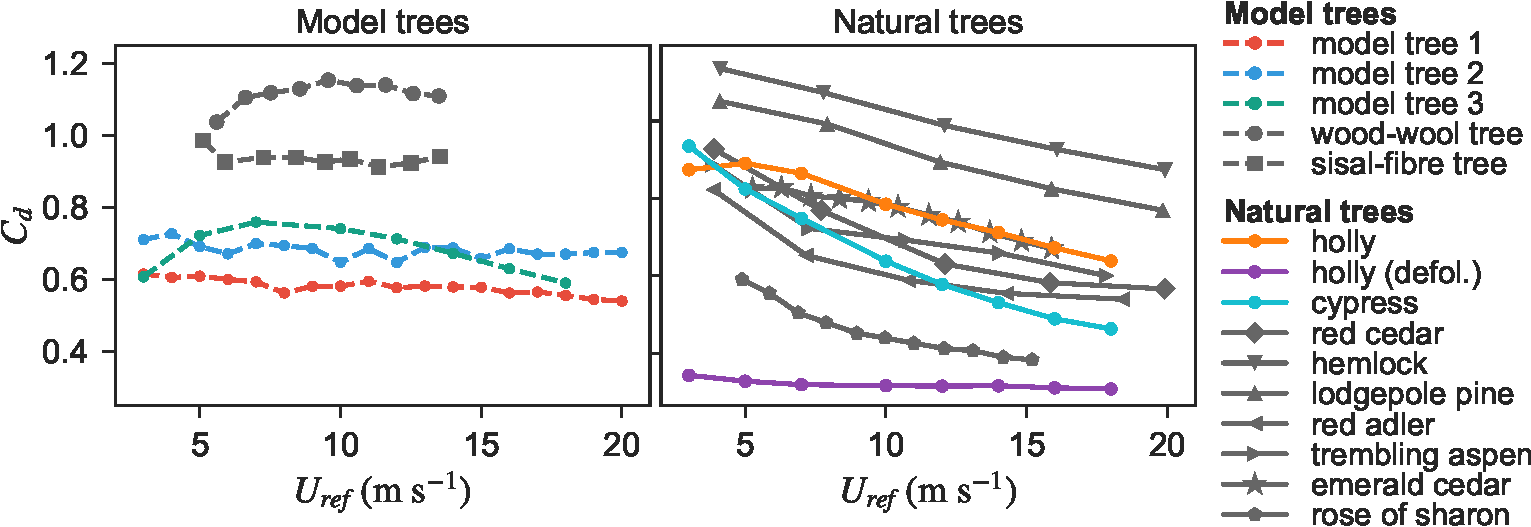
\includegraphics[width=\textwidth]{\figdir/cdvswindspeed_comparison-crop.pdf}
		\caption{Drag coefficient $C_d$ vs. wind speed $U_{\textit{ref}}$ for various model trees (dashed lines) and natural trees (solid lines). The trees of the present study (colored lines) are compared with previous studies results (black lines) as listed in \cref{tab:windtunneltreeslit}.}
		\label{fig:cdvswindspeed}
	\end{figure}

With increasing wind speed, the drag coefficients of model trees 1 and 2 are observed to remain nearly constant, with drag coefficients of around $C_d=0.58$ and $C_d=0.68$, respectively. This constant relationship is also observed for the model wood-wool tree with $C_d=1.12$ and sisal-fibre tree with $C_d=0.94$, studied by \cite{Gromke2008a}. Therefore, drag coefficients of these model trees appear to be independent of wind speed. In contrast, the drag coefficients of all natural trees, and of model tree 3, decrease with wind speed. This dependent behavior could be attributed to the difference in the rigidity of the trees. Due to the higher rigidity of most model trees, they do not undergo a reconfiguration under wind and maintain a constant drag coefficient. In contrast, with the flexible branches and leaves of the natural trees and of model 3, reconfiguration occurs at higher wind speeds, causing a decay of the drag coefficient. Furthermore, the natural trees used in the present study are juvenile indicating a lower moment of elasticity (MOE) \citep{Macdonald2002,Telewski1995,Watt2008}. The reduced MOE and the high foliage density further increases the plant bending at high wind speed. This is especially apparent for the juvenile conifer plant, as observed from \cref{fig:cdvswindspeed}. However, when the tree has no leaves, the reconfiguration of the leaves is no longer present, as seen for the defoliated holly. Therefore, leaves play a critical role in the bending and reconfiguration of the tree. Incorporating the differences in MOE, due to age and the varying foliage density due to season, will lead to more appropriate tree models for wind tunnel measurements. To further understand the influence of reconfiguration, the relationship of drag force with wind speed is investigated in \cref{subsec:reconfiguration}.

\subsection{Influence of porosity on drag coefficient}
\label{subsec:porosity}
\cref{fig:cdvswindspeed} shows that, for a given wind speed, the drag coefficient of model and natural trees can range from $0.25$ and $1.25$. This spread in drag coefficient is also apparent in past studies \citep{Bitog2011,Dong2007,Guan2003,Hagen1971,Vollsinger2005a,Vollsinger2005,Wilson1985}. The spread in drag coefficient of windbreaks and trees is related to the aerodynamic porosity. Using the empirical relation (\cref{eq:aerodynamicporosity}), the drag coefficients of model and natural trees at two Reynolds number are plotted versus aerodynamic porosity, as displayed in \cref{fig:cdvsalpha}. The lower Reynolds number corresponds to $U_{\textit{ref}}=3.0$ to $9.6$ m\,s$^{-1}$ and the higher Reynolds number corresponds to $U_{\textit{ref}}=6.1$ to $19.4$ m\,s$^{-1}$, dependent on the given height of the trees \cref{tab:modeltrees}. The graph also includes the results from the studies cited above. A large spread in the drag coefficient is seen for a given porosity, depending on the tree type. To consider is that the method of calculating the aerodynamic porosity varies across these studies. Some studies rely on optical porosity \citep{Dong2008,Guan2003,Hagen1971,Wilson1985}, others on volumetric porosity \citep{Grant1998} and some determine porosity directly from measuring the bleed flow intensity \citep{Bitog2011}.

	\begin{figure}[t]
	\centering
	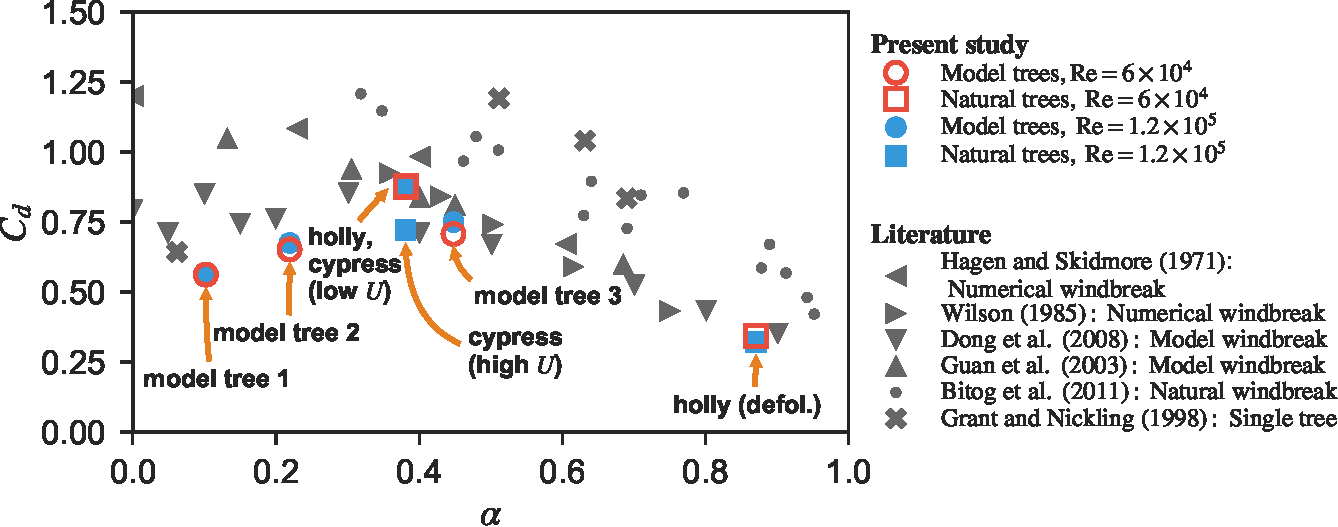
\includegraphics[width=\textwidth]{\figdir/cdvsalpha_type2-crop.pdf}
	\caption{Drag coefficient $C_d$ vs. aerodynamic porosity $\alpha$ for various model trees (model tree 1, model tree 2, model tree 3) and natural trees (holly, cypress, defoliated holly) at two Reynolds number $\mathrm{Re} = \num{6e4}$ and $\mathrm{Re}=\num{1.2e5}$.}
	\label{fig:cdvsalpha}
	\end{figure}

In every study (except \cite{Hagen1971}), the drag coefficient initially increases at low aerodynamic porosity ($\alpha < 0.3$) and decreases at higher aerodynamic porosity ($\alpha > 0.3$). \cite{Dong2007} find $\alpha = 0.3$ to be a critical porosity. Below the critical porosity, the airflow goes primarily around the tree with little bleed flow through the tree, creating in a recirculation zone behind the tree. Above the critical porosity, the bleed flow becomes dominant and, with increasing porosity, the drag exerted by the tree quickly reduces. However, at the critical porosity, a combination of recirculation and bleed flow is present and this additional bleed flow through the foliage seems to result in a larger drag. Therefore, a tree that has this critical porosity, extracts the most momentum from the flow. A similar finding has also been obtained from windbreak studies \citep{Dong2008,Hagen1971,Lee1999}. Finally, the Reynolds number does not have a significant impact on the drag coefficients for most of our measurements, with a variation of about $\pm 4$\%. The cypress of $\alpha=0.381$ has a lower drag coefficient at higher Reynolds numbers, due to the reconfiguration at high wind speeds, as discussed in \cref{subsec:reconfiguration}. Therefore, if the Reynolds number is varied without varying the wind speed, such as by varying the tree height, the Reynolds number will have a weak influence on the drag coefficient. The apparent variation in drag coefficient is manifested only from the reconfiguration of the foliage when the wind speed is high.

\subsection{Influence of plant reconfiguration on drag coefficient}
\label{subsec:reconfiguration}

To study the influence of leaf and branch reconfiguration on the drag coefficient, the drag force-wind speed relationship is examined. The drag force of a tree that reconfigures follows the relationship:
\begin{equation}
F \propto U^{2+b}
\label{eq:vogelrelation}
\end{equation}
where $b$ is called the Vogel exponent, where $b<0$. Its magnitude quantifies the decay of the drag coefficient with wind speed \citep{DeLangre2008,Vogel1989}. The Vogel exponent is more negative for trees that strongly reconfigure. \cite{DeLangre2008} mentions that it is not uncommon to find values of $b=-1$, indicating that the drag force can be linearly dependent on the wind speed. In the present study, we determine the Vogel exponent of the model and natural trees, which have different reconfiguration behavior at high wind speeds, and compare these values with ones of larger trees from previous studies. 

The Vogel exponent of trees from present study and literature are tabulated in \cref{tab:vogelexponents}. The Vogel exponent is determined using a non-linear regression analysis of the modified drag equation (\cref{eq:vogelrelation}). The study confirms that foliated natural trees undergo reconfiguration as mentioned above and seen in \cref{fig:cdvswindspeed}. For natural trees, the Vogel exponent is shown to range from $-0.18$ to $-0.51$. The study also shows that smaller natural trees reconfigure more strongly than larger natural trees possibly due to their thinner branches which can have a lower mechanical stiffness. This is especially apparent for cypress with a Vogel exponent of $b=-0.51$. In contrast, the Vogel exponent of the defoliated holly is $-0.05$, showing a lack of reconfiguration as observed in \cref{fig:cdvswindspeed}. The study highlights the influence of leaves in reconfiguration and how reconfiguration dynamically affects the drag coefficient.

{
	\ctable[
	caption = {The Vogel exponent $b$ of model and natural trees.},
	label   = {tab:vogelexponents},
	pos = t,
	mincapwidth = \textwidth,
	]{lrp{1cm}lr}{ $^{a}$\cite{Gromke2008a}, $^{b}$\cite{Vollsinger2005a}, $^{c}$\cite{Vollsinger2005}
	}{
		
		\FL
		\multicolumn{2}{c}{\textit{Present study}} & & \multicolumn{2}{c}{\textit{Literature}} \\
		Name	 				& 	$b$ & & Name & $b$
		\ML
		\multicolumn{5}{c}{\textit{Model trees}} \\
		model tree 1 & $-0.12$	& & wood-wool tree$^a$ & $-0.02$ \\
		model tree 2 & $0$\quad\,\, & & sisal-fiber tree$^a$ & $0$\quad\,\, \\
		model tree 3 & $-0.33$  & &   & \\[7pt]
		\multicolumn{5}{c}{\textit{Natural trees}} \\
		holly 		 & $-0.33$  & & red cedar$^b$ & $-0.25$ \\
		holly (defol.) & $-0.05$ & & hemlock$^b$ & $-0.23$ \\
		cypress 	& $-0.51$   & & lodgepole pine$^b$ & $-0.28$ \\ 		 		
		&  			& & red adler$^c$	& $-0.18$ \\
		&  			& & trembling aspen$^c$	& $-0.26$	 			
		\LL}
}

Model trees, in general, show less reconfiguration and, as consequence, the Vogel exponent is less negative except for model tree 3. The model tree 3 has a Vogel exponent $b=-0.33$, so equal to that of holly, due to its similar reconfiguration characteristic, and displays as a result a decaying drag coefficient as shown in \cref{fig:cdvswindspeed}. In contrast, rigid model trees, such as model tree 2 do not behave similarly to the way natural trees do.


\section{Impact on mean wind speed}

The normalized mean velocity magnitude $\tavg{\mvec{u}}/U_{\textit{ref}}$ provides a first indication of the influence of trees on the airflow. The wind speed is normalized by the reference wind speed $U_{\textit{ref}}$, determined at the location of the tree before its placement. To allow comparison, all trees are subjected to a similar uniform velocity profile, as explained above. \cref{fig:unorm} compares the normalized mean wind speed of model and natural trees at two distinct wind speeds, i.e. at low, $U_{\textit{ref}}=1$, and high, $U_{\textit{ref}}=10$ m\,s$^{-1}$, wind speeds. The figure shows that the wake flow field differs from tree to tree and varies with wind speed. This behavior is directly related to the variation in the aerodynamic porosity with wind speed, which is evaluated as follows. The aerodynamic porosity of the measured 2D-PIV plane is directly determined from the ratio of the bleed wind speed and the upstream wind speed \citep{Guan2003}:
\begin{equation}
\alpha^{\mathrm{2D}} = \frac{\int\limits_0^H { |{\tavg{\mvec{u}}}|\,\mathrm{d}z}}{U_{\textit{ref}} \, H}
\label{eq:2dporosity}
\end{equation}
measured at $x/H=0.7$. This location is chosen as it is the closest point to the tree where the measured wake velocity distribution of all the trees is available. Ideally, the bleed flow behind the tree should be measured as close to the tree as possible. The measured 2D-plane aerodynamic porosity is indicated in \cref{fig:unorm} and represents the effect of the porosity at the measured plane, whereas $\alpha$ is the empirically-determined aerodynamic porosity of the entire tree. Furthermore, the measured 2D-plane aerodynamic porosity is dependent on the wind speed and therefore takes into account the influence of reconfiguration.

	\begin{sidewaysfigure}[p]
	\centering
	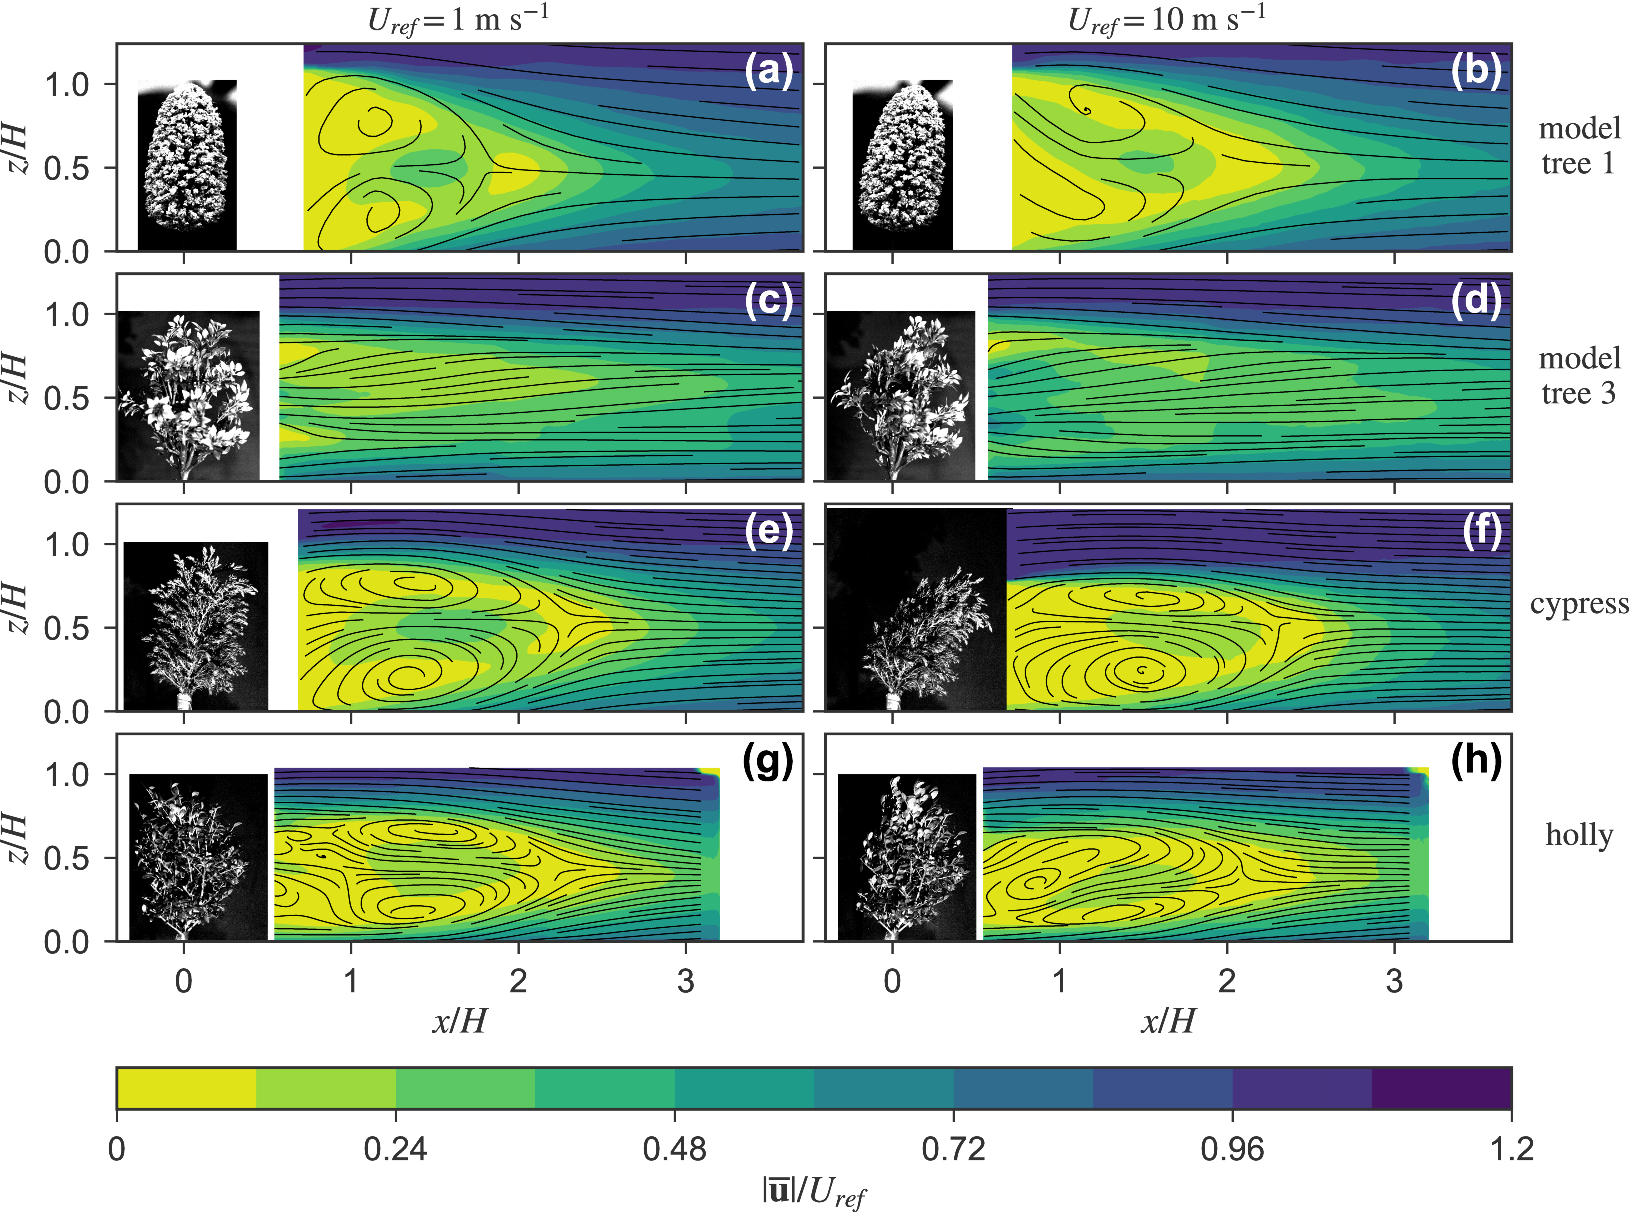
\includegraphics[height=0.7\textheight]{\figdir/unorm-eps-converted-to.pdf}
	\caption{Normalized mean velocity magnitude $|\tavg{\mvec{u}}|/U_{\textit{ref}}$ of \subfig{a}\subfig{b} model tree 1, \subfig{c}\subfig{d} model tree 3, \subfig{e}\subfig{f} cypress, \subfig{g}\subfig{h} holly. The comparison is done for two wind speeds: \subfig{a}\subfig{c}\subfig{e}\subfig{g} $U_{\textit{ref}}=1$ m\,s$^{-1}$ and \subfig{b}\subfig{d}\subfig{f}\subfig{h} $U_{\textit{ref}}=10$ m\,s$^{-1}$.}
	\label{fig:unorm}
	\end{sidewaysfigure}

\cref{fig:unorm}a-b shows model tree 1 with a strong recirculation, as shown by the appearance of closed streamlines. The 2D-plane aerodynamic porosity of model tree 1 is shown to be substantially lower than that of model tree 3 and of holly. The cypress tree shows a similar wake flow field due to its low porosity. An increase in wind speed results in bending of both the model tree 1 and the cypress. However, the reconfiguration of the trees has a dissimilar effect, where the 2D-plane porosity of model tree 1 increases with wind speed while that of the cypress tree is reduced. This occurs because, unlike model tree 1, the cypress tree has flexible foliage and higher wind speed results in the foliage of the cypress tree to reconfigure into a smaller clump, resulting in a stronger blockage. In contrast, the model tree 3 shows strong bleed flow due to its higher aerodynamic porosity. Furthermore, the bleed flow increases with wind speed, as indicated by the increase of both 2D-plane aerodynamic porosity by $0.115$ and wind speeds in the wake. The holly only shows bleed flow where it has a higher porosity, i.e. in its top part. Below, due to the higher foliage density of holly, strong recirculation is evident. In all cases, the impact of reconfiguration is evident, showing an altered wake structure and changing aerodynamic porosity at higher wind speeds. The comparison highlights the implication of reconfiguration on the wake. This change is also reflected in the drag coefficient measurements as seen in \cref{fig:cdvswindspeed}.

\section{Impact on turbulence intensity}

The influence of trees on the fluctuating component of the wind is studied by quantifying the change in local turbulence intensity $I$, defined as
\begin{equation}
I = \frac{\sqrt{2/3\,k}}{|\tavg{\mvec{u}}|}
\end{equation}	
where $|\tavg{\mvec{u}}|$ is the mean local wind speed and
\begin{equation}
k = \frac{1}{2} \mathrm{tr} \left(\tavg{\mvec{u}'\mvec{u}'}\right)
\end{equation}
and we approximated lateral variance with the assumption that
\begin{equation}
\tavg{v'v'} = \frac{1}{2}\left(\tavg{u'u'} + \tavg{w'w'}\right)
\end{equation}

The turbulence intensity measures the ratio of the fluctuating velocity to the local mean velocity. \cref{fig:ti} shows the turbulence intensity for the model and natural trees at low and high wind speeds. The comparison of the results for model and natural trees shows that the turbulence intensity distribution of model tree 1 resembles the most that of natural trees. Due to the much higher bleed flow of model tree 3, as observed in \cref{fig:unorm}, the turbulence intensity rise in the wake is much lower, with an average local turbulence intensity of less than $20$\%.

	\begin{sidewaysfigure}[p]
	\centering
	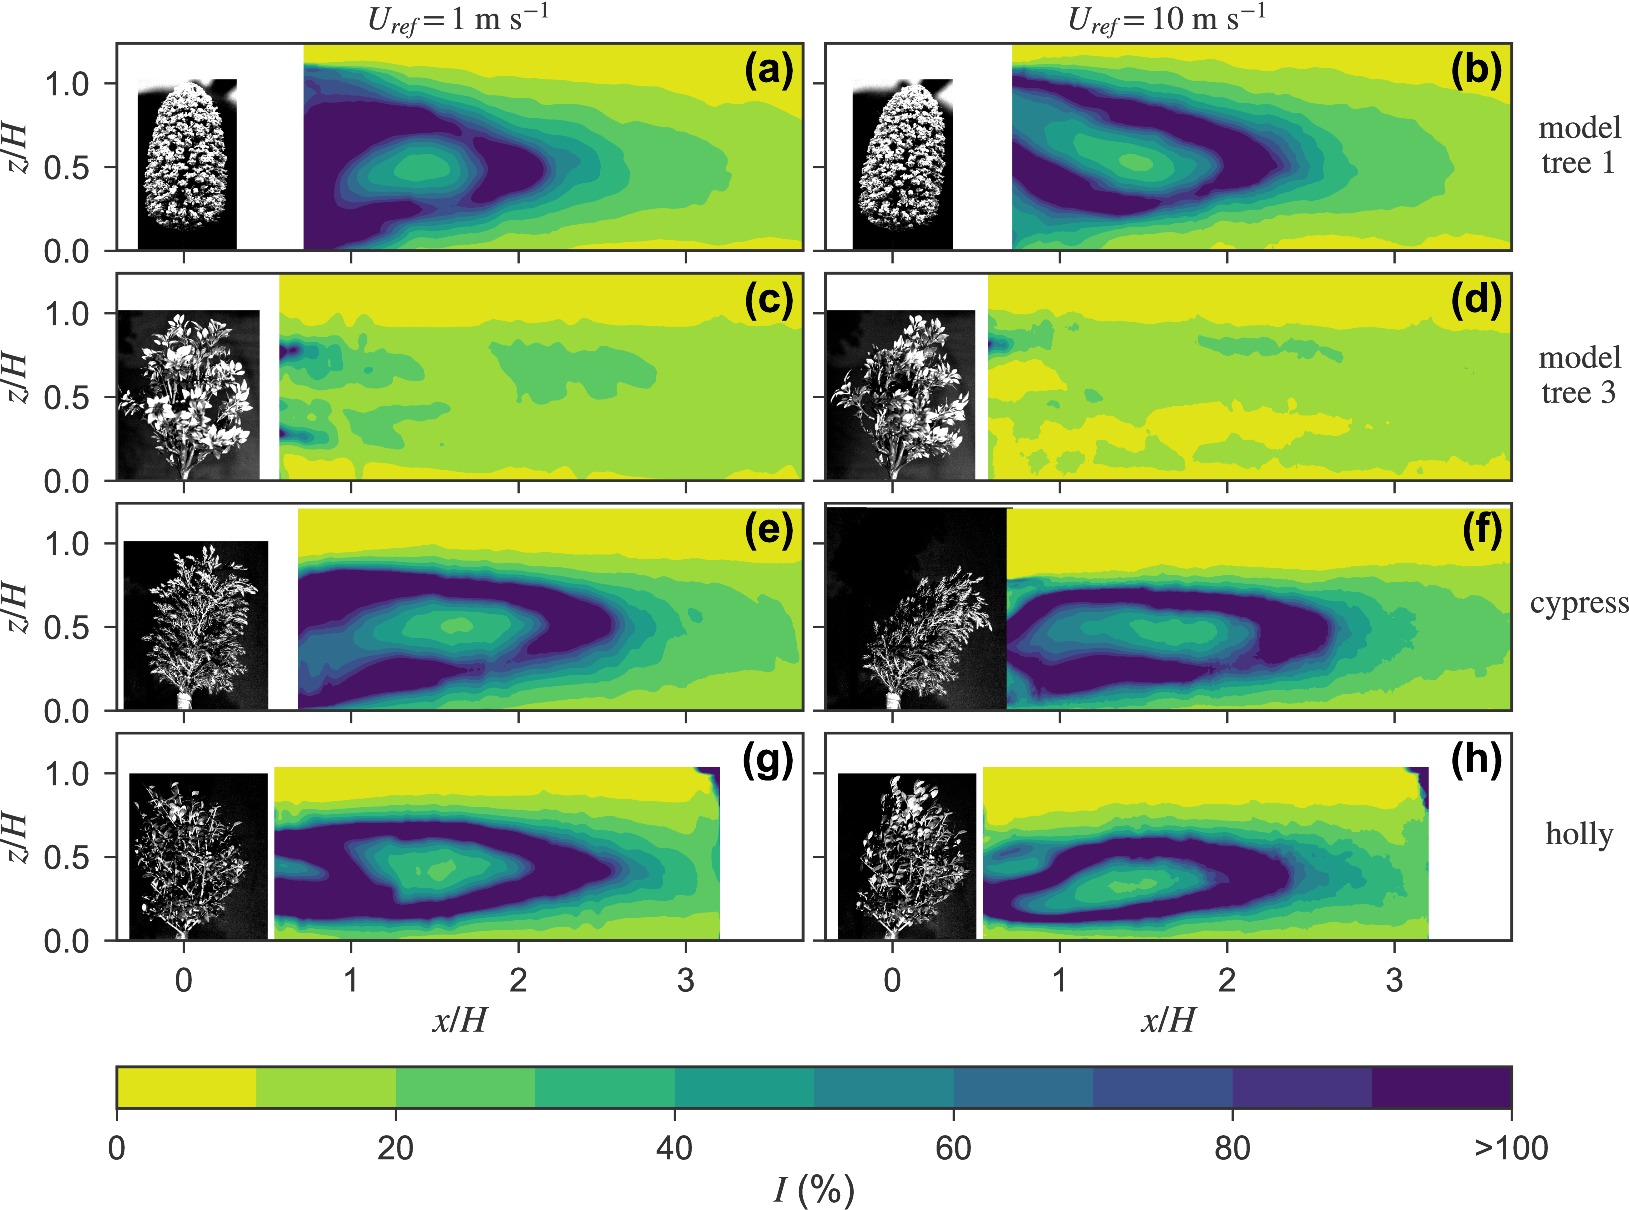
\includegraphics[height=0.7\textheight]{\figdir/ti_local-eps-converted-to.pdf}
	\caption{Turbulence intensity $I=\sqrt{2/3 k}/\tavg{\mvec{u}}$ (\%) of \subfig{a}\subfig{b} model tree 1, \subfig{c}\subfig{d} model tree 3, \subfig{e}\subfig{f} cypress and \subfig{g}\subfig{h} holly. The comparison is done for two wind speeds: \subfig{a}\subfig{c}\subfig{e}\subfig{g} $U_{\textit{ref}}=1$ m\,s$^{-1}$ and \subfig{b}\subfig{d}\subfig{f}\subfig{h} $U_{\textit{ref}}=10$ m\,s$^{-1}$.}
	\label{fig:ti}
	\end{sidewaysfigure}

Comparing low to high wind speeds shows how reconfiguration due to bending of the trees influences the turbulence in the wake. Model tree 1 (\cref{fig:ti}b) and cypress tree (\cref{fig:ti}f) bend at high wind speeds, as reflected in a weak change in the turbulence intensity distribution. Only in the near vicinity of the trees, a noticeable change is observed, showing a reduction in the size of the high turbulence intensity region. The influence of reconfiguration due to streamlining of the branches and leaves on the turbulence intensity is observable for model tree 3 and the hardwood holly tree. In the case of model tree 3, the turbulence intensity is seen to reduce, as a result of the increase in aerodynamic porosity of $\Delta \alpha^{\textit{2D}} = 0.115$, as observed in \cref{fig:unorm}d. In the case of holly tree, the turbulence intensity is only found to increase at the near-wake region ($x/H<1$), with an increase in aerodynamic porosity of only $\Delta \alpha^{\textit{2D}} = 0.07$. Therefore, the influence of reconfiguration on the turbulence intensity is strongly influenced by the nature of reconfiguration and varies from species to species.


\section{Impact on Sheltering effect}

The sheltering provided by the trees is known to be related to the shape, porosity and flexibility of the tree. It can be assessed by determining the shelter parameter $\psi$, given as \citep{Gandemer1979}:
\begin{equation}
\psi  = \frac{{{U_{\textit{ref}}} + \sqrt {\frac{2}{3} {k_{\textit{ref}}}} }}{{ |\tavg{\mvec{u}}| + \sqrt {\frac{2}{3} k} }}
\end{equation}

The shelter parameter takes in account the mean velocity and its fluctuating component, thereby quantifying the net reduction in wind speed. Similar formulations of the shelter effect are found in previous studies \citep{Lee2014565,Lee2012,McClure2017,Packwood2000,Perera1981,Santiago2007}. The shelter parameter provides a distinction between regions of high sheltering ($\psi \gg 1$) and no sheltering ($\psi \approx 0$).

	\begin{sidewaysfigure}[p]
	\centering
	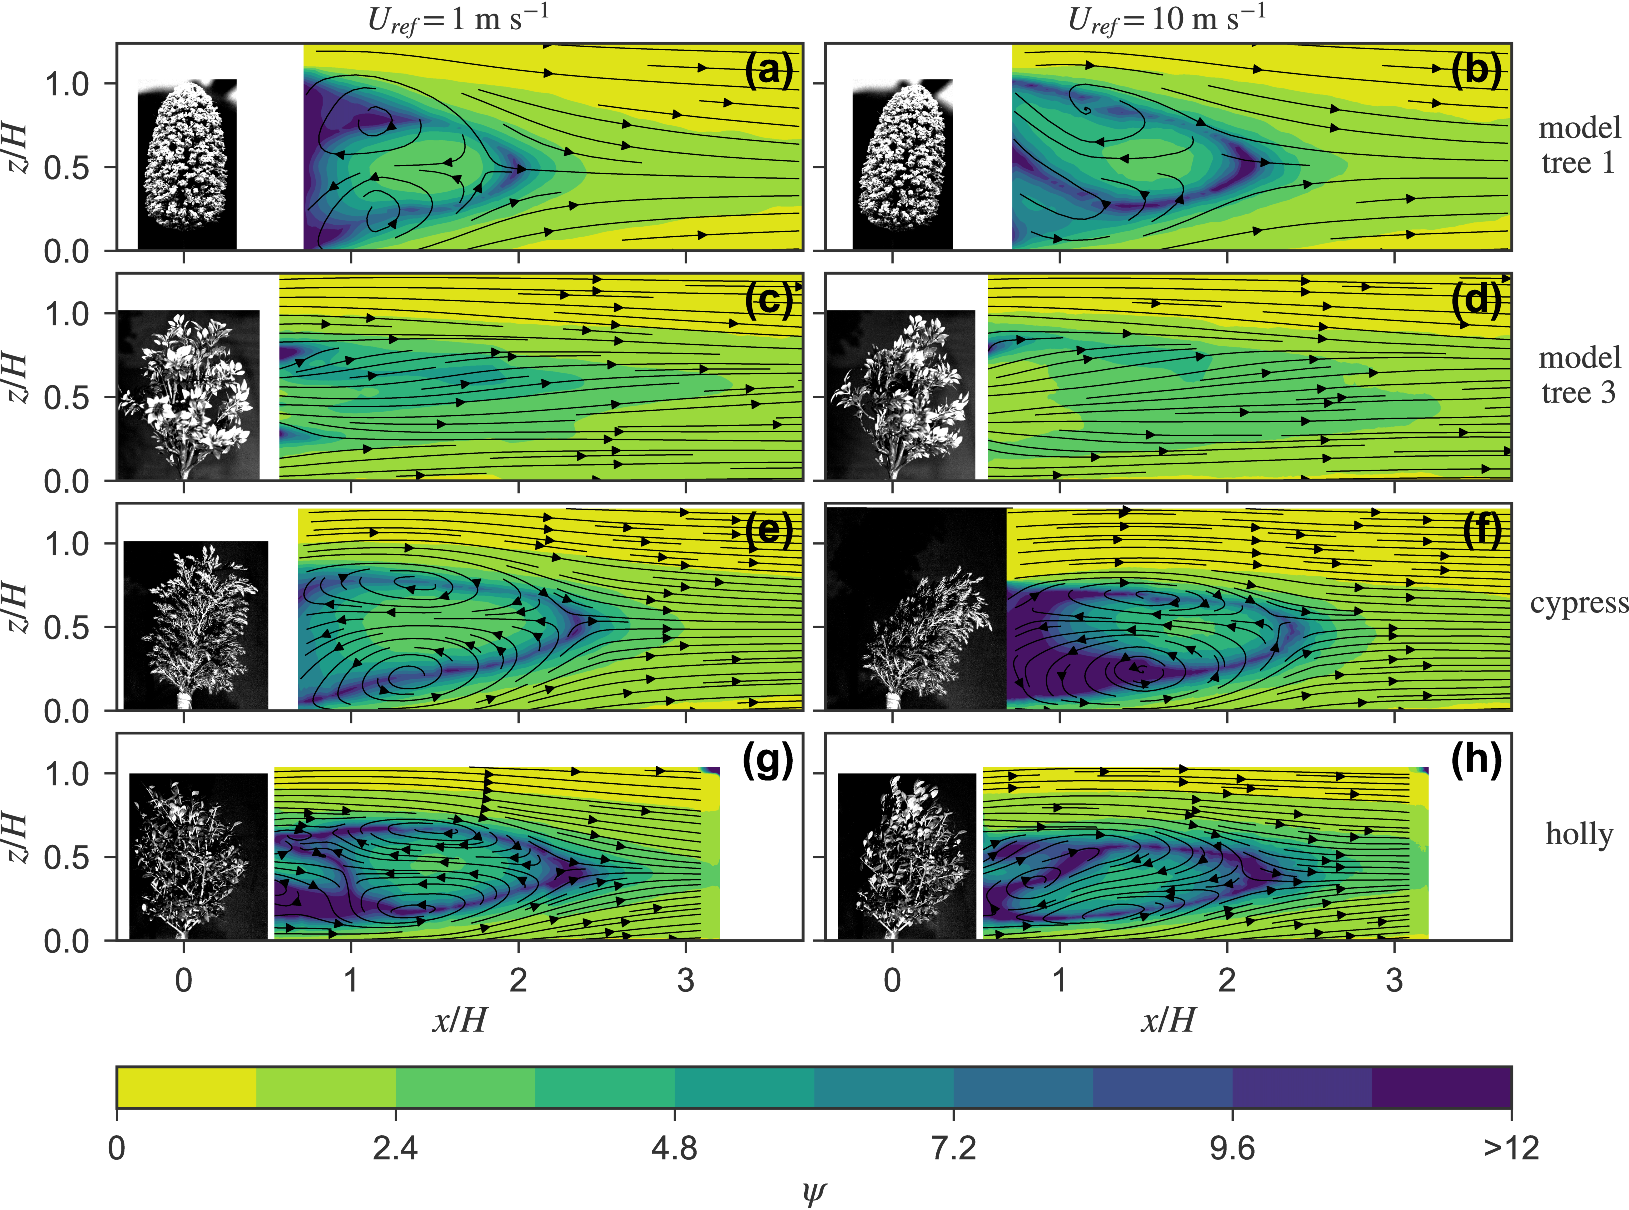
\includegraphics[height=0.7\textheight]{\figdir/psi_v2-eps-converted-to.pdf}
	\caption{Shelter parameter $\psi$ of \subfig{a}\subfig{b} model tree 1, \subfig{c}\subfig{d} model tree 3, \subfig{e}\subfig{f} cypress and \subfig{g}\subfig{h} holly. The comparison is done for two wind speeds: \subfig{a}\subfig{c}\subfig{e}\subfig{g} $U_{\textit{ref}}=1$ m\,s$^{-1}$ and \subfig{b}\subfig{d}\subfig{f}\subfig{h} $U_{\textit{ref}}=10$ m\,s$^{-1}$.}
	\label{fig:psi}
	\end{sidewaysfigure}


\cref{fig:psi} compares the shelter parameter of four trees at $U_{\textit{ref}}=1$ and $10$ m\,s$^{-1}$. Generally, the highest sheltering is provided at the near-wake region ($x/H<1$), showing highest intensity of $\psi$ . Increasing the wind speed only results in a slight change in the shelter parameter for most trees, except for cypress which shows a substantial increase in sheltering. Model tree 3 shows a decrease in sheltering. Model tree 3 shows that, due to the increased bleed flow caused by streamlining of branches and leaves, the sheltering is slightly reduced. The shelter parameter varies with the change in aerodynamic porosity. Thus, the reconfiguration of the tree has a direct influence on the sheltering provided by the tree.

\section{Influence of seasonal foliar density variation}

The seasonal foliar density variation evidently affects the flow field with deciduous trees as they which shed their leaves during winter. This influence of the seasonal change of tree foliage on the flow field is illustrated here by comparing the same holly in foliated and defoliated states. \cref{fig:psileafless} shows the shelter parameter and streamlines of holly with and without leaves at a high wind speed ($U_{\textit{ref}}=10$ m\,s$^{-1}$). In leafless configuration (\cref{fig:psileafless}b), the tree has a negligible influence on the flow whereas the foliated holly shows strong sheltering and recirculation in the wake (\cref{fig:psileafless}a). This variation is also quantified by the substantial increase in the 2D-plane aerodynamic porosity $\alpha^{2D}$ from \numrange{0.315}{0.775} and results in a substantial drop of drag coefficient of the tree (\cref{fig:cdvswindspeed}). The measurement shows that the drag coefficient of defoliated holly is significantly lower than that of the foliated configuration. 

	\begin{figure}[t]
	\centering
	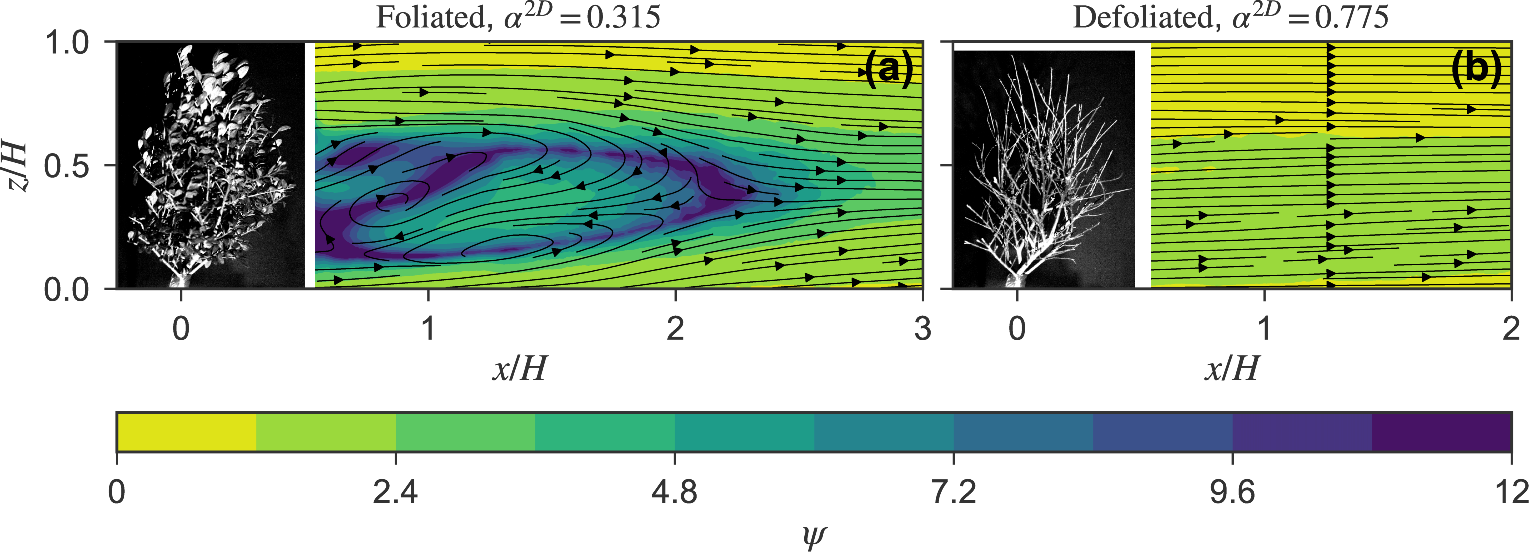
\includegraphics[width=\textwidth]{\figdir/psi_leafless_v2-eps-converted-to.pdf}
	\caption{Shelter parameter $\psi$ of \subfig{a} foliated holly and \subfig{b} defoliated holly at $U_{\textit{ref}}=10$ m\,s$^{-1}$.}
	\label{fig:psileafless}
	\end{figure}

Extrapolating from these results, deciduous trees can be assumed to have a negligible impact on the airflow during winter seasons. Therefore, to accurately model the impact of vegetation, urban microclimate models should be able to take in account this annual variation of aerodynamic porosity and the resulting change in turbulence statistics of the tree wake.

\section{Conclusion}

The present study compares the aerodynamic performance of model trees and natural trees using drag force measurements and PIV (Particle Image Velocimetry) measurements. The drag force measurements show that the behavior of natural trees can be approximated by model trees only if they have a similar aerodynamic porosity and if they are capable of reconfiguring at high wind speeds. However, the PIV measurements showed that the model tree 1, which has a low porosity, had a wake structure similar to the one of the natural cypress tree. Model tree 3, with foliage consisting of individual polymeric thin leaves, reconfigures in a way similar to that of natural hardwood tree. Although, in the present study, it is evident that the model tree 3 has a much higher aerodynamic porosity than the natural tree resulting in a dominant bleed flow. In contrast, model tree 1 and the natural trees indicated strong recirculation due to their lower aerodynamic porosity.

The influence of foliage reconfiguration where the branches and the leaves deform due to airflow is evident in both the drag-velocity measurements and also from PIV measurements of the wake region. Due to reconfiguration, the drag coefficient decays at high wind speeds. The natural trees and the model tree 3 with artificial leaves show reconfiguration and a linear drag-force-wind speed relationship. A study on the Vogel exponent identifies the strength of the reconfiguration and shows that small young natural trees reconfigure to a larger extent than larger mature trees do. Therefore, future studies should focus on directly quantifying foliage deformation and its correlation to the resulting flow field.

In addition to reconfiguration, the aerodynamic porosity of the trees plays a critical role in their drag behavior, as reflected by the drag coefficient. In contrast, the Reynolds number only has an influence on the drag coefficient of the trees due to the influence of wind speed on reconfiguration. From the PIV measurements, it is apparent that the aerodynamic porosity, as determined from the optical porosity, does not reflect the aerodynamic porosity of the measured 2D-PIV plane. The 2D-plane aerodynamic porosity is shown to be dependent on the wind speed as the reconfiguration of the foliage directly influences the aerodynamic porosity. Due to reconfiguration, the turbulence intensity and shelter parameter are shown to be dependent on the wind speed.

The study of seasonal foliar density variation by comparing the holly in foliated and defoliated state shows that, during winter seasons, the influence of deciduous trees on the flow can be assumed to be negligible. Therefore, neglecting deciduous trees during winter in urban microclimate models can be a valid assumption and an advantage towards computational efficiency. In contrast, coniferous trees and evergreen hardwood trees that do not shed leaves and instead maintain their foliage density, annually, still provide sheltering during winter seasons and therefore their influences must be taken into account over all seasons.

In conclusion, towards the design, development or use of model trees for wind tunnel studies, the aerodynamic porosity and the drag coefficient are seen as vital parameters that should be matched to those of the natural trees of interest. When studying the influence of reconfiguration of the plant on the flow field, the Vogel exponent of the model tree is the recommended parameter to compare to the natural tree. Finally, if the objective of the wind tunnel experiment is to study the sheltering characteristics of the plant, the shelter parameter is the one to focus on. However, this requires a direct measurement of the wake flow field using more advanced techniques, such as PIV or hot-wire measurements, which might not be easily available.

